\chapter{Метод автоматического перебора расширенных моделей с разным числом параметров и настройки параметров по генетическим данным одной, двух и трех популяций}
\label{ch:auto_model}

Классические методы вывода демографической истории популяций предполагают использование параметризованной модели демографической истории.
Для более надежного результата требуется вручную перебирать множество моделей и выбирать ту, которая наилучшим образом описывает генетические данные.
В данной работе был разработан класс расширенных моделей, которые включают параметры динамики изменения численности для настройки и уже элиминируют часть этого перебора.
Следующим шагом в автоматизации всего процесса вывода демографической истории популяции является метод автоматического перебора моделей расширенного класса.

В данной главе представлено описание разработанного метода автоматического перебора моделей, а также результаты экспериментальных исследований на реальных данных.

\section{Метод автоматического перебора моделей расширенного класса}

Был разработан метод автоматического перебора моделей расширенного класса.
Пользователю необходимо лишь задать минимальные и максимальные ограничения на модель и метод самостоятельно выполнит перебор моделей расширенного класса в предоставленных границах.

\subsection{Разработка метода автоматического перебора моделей расширенного класса}

На каждой итерации разработанный метод использует метод настройки параметров на основе комбинации глобальной и локальной оптимизации --- разработанный комбинированный метод на основе генетического алгоритма и метода BFGS.
Метод начинает с создания и настройки расширенной модели, которая удовлетворяет входным минимальным ограничениям.
Затем на каждой итерации текущая модель изменяется, увеличивается число ее параметров, и снова запускается процесс настройки ее параметров по генетическим данным.
При достижении максимальных ограничений на модели, метод останавливается и происходит сравнение всех перебранных моделей с помощью информационного критерия Акаике.
В результате работы, выбирается настроенная модель, которая наилучшим образом описывает генетические данные.
Таким образом, можно описать следующие шаги разработанного метода:
\begin{enumerate}
    \item Создать текущую модель, как модель с минимальными ограничениями.
    \item Настроить параметры для текущей модели по генетическим данным.
    \item Создать следующую модель, подходящую под ограничения.
    \item Повторить пункты б), в) пока не будут достигнуты максимальные ограничения.
    \item Сравнить множество перебранных моделей и выбрать лучшую.\\
\end{enumerate}
Блок-схема разработанного метода представлена на рисунке~\ref{fig:auto:scheme}.
Псевдокод метода представлен в листинге~\ref{alg:part4:auto_search}.
На вход метод получает генетические данные $\mathfrak{D}$, метод вычисления правдоподобия $f_{\mathcal{M}}$, минимальные, максимальные ограничения моделей $S_{\min}$, $S_{\max}$ соответственно и набор констант $B$, который задает какие параметры включены в модели и будет определен далее.\\

%Алгоритм выглядит следующим образом:
\begin{figure}[ht!]
    \centering
    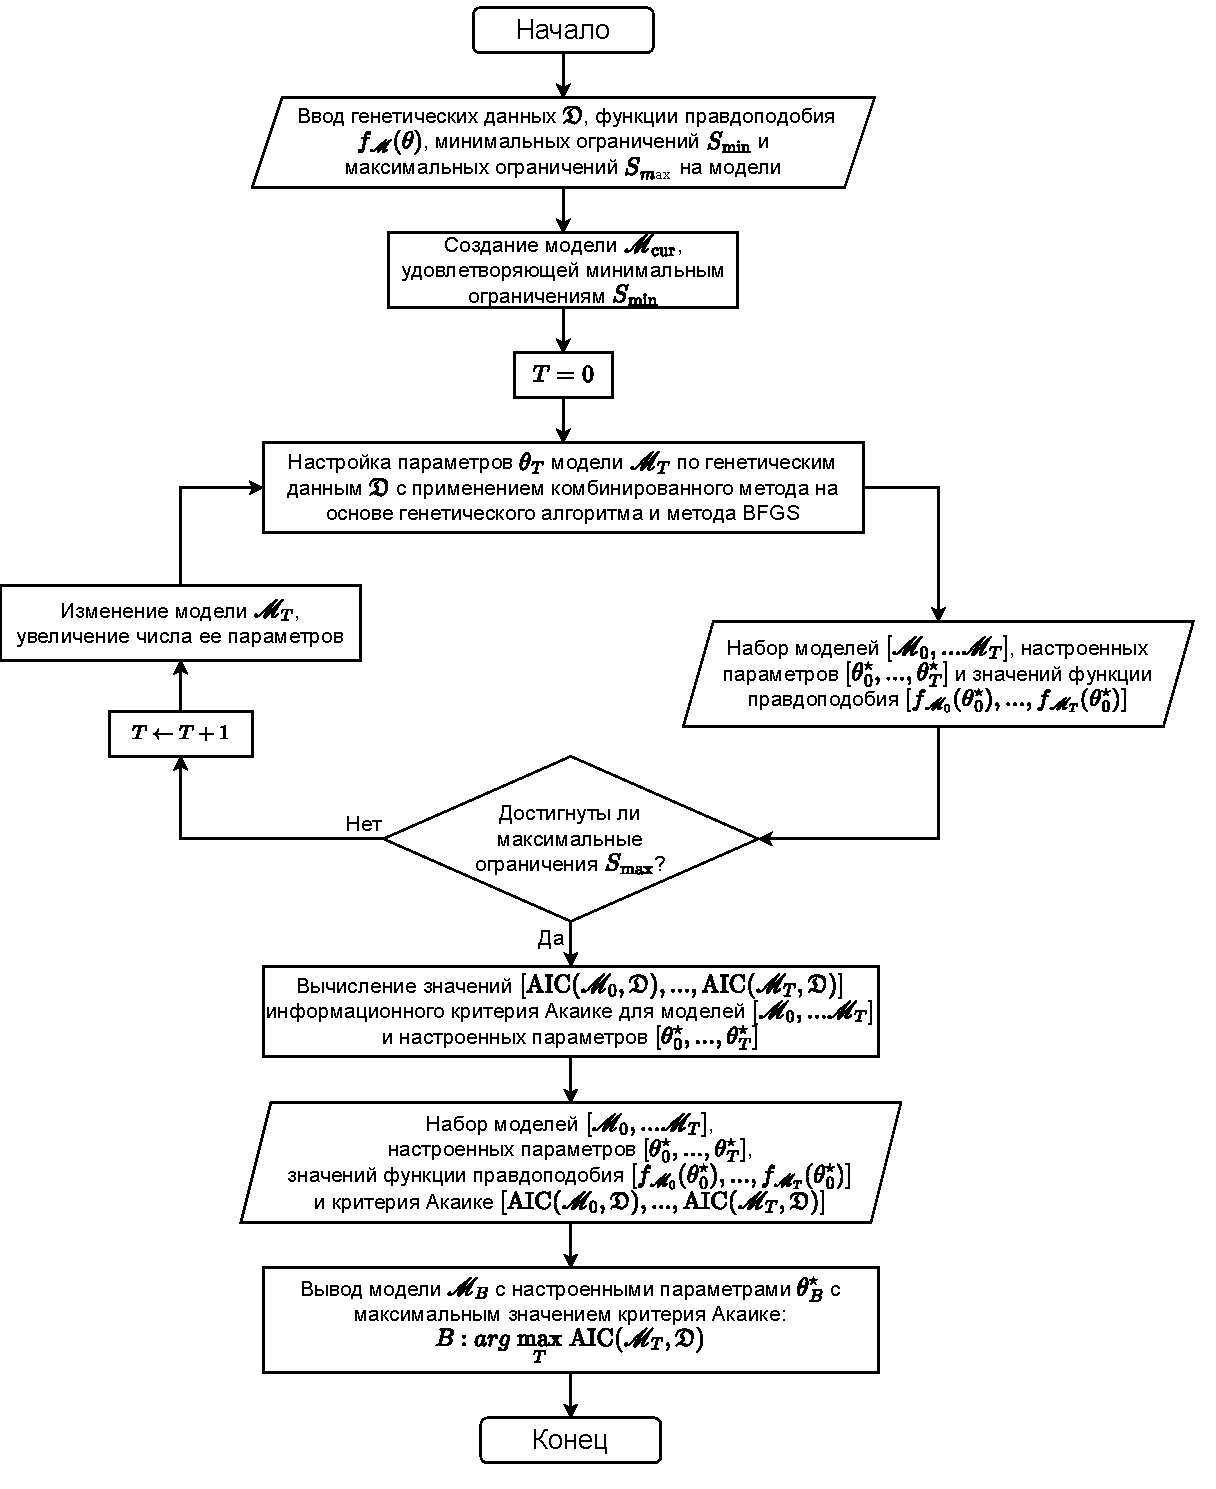
\includegraphics[width=\linewidth]{images/part4/auto_model.drawio.pdf}
    \caption{Блок-схема разработанного метода автоматического перебора моделей расширенного класса с разным числом параметров}
    \label{fig:auto:scheme}
\end{figure}

\begin{algorithm}
\caption{Процедура автоматического перебора моделей демографической истории популяций по генетическим данным}
\label{alg:part4:auto_search}
\begin{algorithmic}[1]
\Function{GetBestDemographicHistory}{$\mathfrak{D}, f_\mathcal{M}, S_{\min}, S_{\max}, B$}
\State {$\text{results} \leftarrow [\,]$}
\State {$S_{\text{cur}} \leftarrow S_{\min}$}
\State {$\mathcal{M} \leftarrow \Call{GetModelFromS}{S_{\min}, B}$}
\State {$\theta^\star \leftarrow \Call{GetBestParams}{f_\mathcal{M}, \mathfrak{D}}$}
\State {$\text{results}[S_{\min}] \leftarrow \theta^*$}
\While{$S_{\text{cur}} \neq S^F$}
    \State {$\mathcal{M}, \theta_\text{cur}, S_{\text{cur}} \leftarrow \Call{ChangeModel}{\mathcal{M}, \theta^*, S_{\text{cur}}, S_{\max}, B}$}
    \State {$\text{results}[S_{\text{cur}}] \leftarrow \Call{GetBestParams}{f_\mathcal{M}, \mathfrak{D}, \theta_\text{cur}}$}
\EndWhile
\State \Return $\Call{BestByAIC}{\text{results}, f_\mathcal{M}, \mathfrak{D}}$
\EndFunction
\end{algorithmic}
\end{algorithm}

На вход:
\begin{itemize}
    \item генетические данные и информация о наличии зависимости в данных;
    \item метод вычисления правдоподобия;
    \item условия-ограничения для расширенных моделей.
\end{itemize}

На выход:
\begin{itemize}
    \item множество моделей, подходящих под условия-ограничения, и их настроенные значения параметров;
    \item выбор лучшей модели с использованием критерия Акаике~\cite{akaike1974new}\cite{coffman2016computationally}.\\
\end{itemize}

\textbf{Задание ограничений на модели.}
Для использования метода автоматического перебора требуется определить ограничения на модели.
Для задания ограничений модели предлагается использовать число временных интервалов:
\begin{itemize}
    \item будем рассматривать максимум три популяции. В случае одной популяции в модели не будет разделения, в случае двух популяций будет одно разделение популяций и в случае трех популяций --- два разделения;
    \item будем задавать три числа $S=\{s_1, s_2, s_3\}$. Первое число $s_1$ определяет число временных интервалов до первого разделения (включая самый первый бесконечный интервал), второе число $s_2$ задает число временных интервалов между первым и вторым разделением, последнее третье число $s_3$ равно числу временных интервалов после второго разделения.
\end{itemize}

Дополнительно определим набор булевых констант $B$:
$$B=\{b_\text{mig}, b_\text{sym\_mig}, b_\text{inbr}, b_\text{const}, b_\text{lin}, b_\text{exp}\},$$
которые задают какие параметры включены в модели.
Например, если $b_\text{mig}$ истинна, то модель содержит параметры миграции для каждого временного интервала. В противном случае в модели отсутствуют параметры миграции.
Обозначенные константы соответствуют следующим параметрам и применимы для всех временных интервалов модели одновременно:
\begin{itemize}
    \item $b_\text{mig}$ обозначает наличие или отсутствие параметров миграции;
    \item $b_\text{sym\_mig}$ определяет являются ли миграции симметричными или асимметричными --- задаются разными параметрами;
    \item $b_\text{inbr}$ определяет наличие или отсутствие параметров инбридинга;
    \item $b_\text{const}$ определяет включена ли постоянная динамика численности в область определения параметров динамики;
    \item $b_\text{lin}$ определяет включена ли линейная динамика численности в область определения параметров динамики;
    \item $b_\text{exp}$ определяет включена ли экспоненциальная динамика численности в область определения параметров динамики.
\end{itemize}

\definition Ограничение модели --- три числа $S=\{s_1, s_2, s_3\}$ временных интервалов.\\

Для заданного ограничения $S=\{s_1, s_2, s_3\}$ и набора булевых констант $B$ модель расширенного класса создается автоматически со всеми возможными параметрами, включая динамики изменения численности.
Минимальное ограничение моделей --- это минимальное $S_{\min}=\{s_1, s_2, s_3\}$ число  временных интервалов в модели, максимальное ограничение --- это максимально возможное $S_{\max}=\{s_1, s_2, s_3\}$ число временных интервалов в модели.
Набор булевых констант $B$, которые задают параметры моделей.
Например, если $b_\text{mig}$, остается зафиксированным во время метода автоматического перебора моделей.

Ограничение включает три числа, так как разработанный метод применим только для одной, двух или трех популяций. Пример модели, соответствующей ограничению (2,1,1), представлен на рисунке~\ref{fig:auto:struct_2_1_1}.
\begin{figure}[ht]
    \centering
    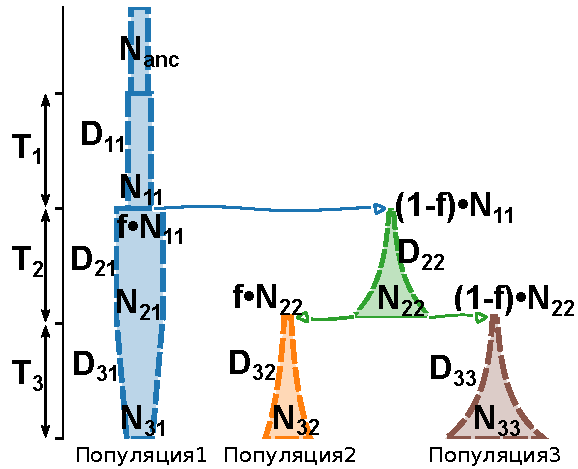
\includegraphics[width=0.6\linewidth]{images_2/struct_2_1_1.pdf}
    \caption{Пример модели трех популяций, которая соответствует ограничению~(2,1,1)}
    \label{fig:auto:struct_2_1_1}
\end{figure}

Пример модели двух популяций для структуры~(2,1,0) представлен на рисунке~\ref{fig:auto:struct_2_1_0}.
На рисунке~\ref{fig:auto:struct_2_1_0_ex} приведены демографические истории, которые соответствуют модели со следующими значениями параметров:
\begin{enumerate}
    \item \texttt{Nanc}: 7200, \texttt{T1}: 30000, \texttt{N11}: 40000, \texttt{D11}: Lin, \texttt{f}: $0.8$, \texttt{T2}: 50000, \texttt{N21}: 500, \texttt{N22}: 500, \texttt{D21}: Exp, \texttt{D22}: Sud;
    \item \texttt{Nanc}: 40000, \texttt{T1}: 50000, \texttt{N11}: 7000, \texttt{D11}: Sud, \texttt{f}: $0.1$, \texttt{T2}: 50000, \texttt{N21}:~5000, \texttt{N22}: 5000, \texttt{D21}: Lin, \texttt{D22}: Exp;
    \item \texttt{Nanc}: 7000, \texttt{T1}: 40000, \texttt{N11}: 20000, \texttt{D11}: Sud, \texttt{f}: 0.2, \texttt{T2}: 80000, \texttt{N21}:~20000, \texttt{N22}: 500, \texttt{D21}: Exp, \texttt{D22}: Lin.\\
\end{enumerate}

\begin{figure}[ht]
    \centering
    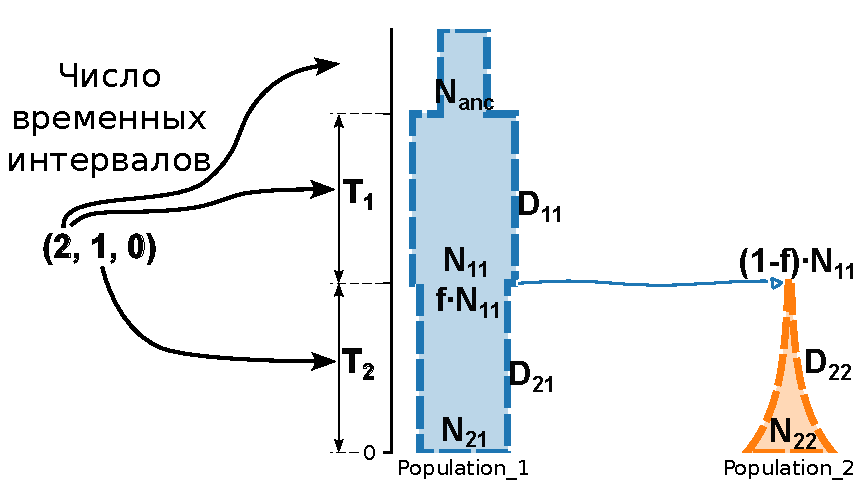
\includegraphics[width=0.6\linewidth]{images_2/picture_2pops_str_base.pdf}
    \caption{Пример модели двух популяций, соответствующей ограничению~(2,1,0)}
    \label{fig:auto:struct_2_1_0}
\end{figure}

\begin{figure}[ht]
    \centering
    \begin{subfigure}[c]{.32\textwidth}
    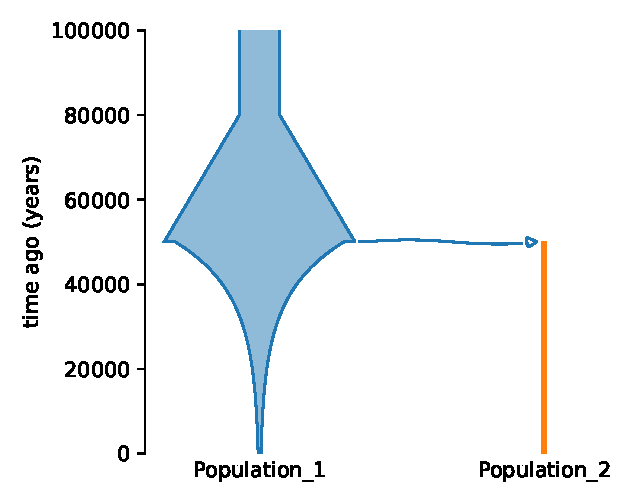
\includegraphics[width=\textwidth]{images_2/picture_2pops_str_2.pdf}
    \caption{}
    \label{fig:auto:struct_2_1_0_ex_1}
    \end{subfigure}%
    \begin{subfigure}[c]{.32\textwidth}
    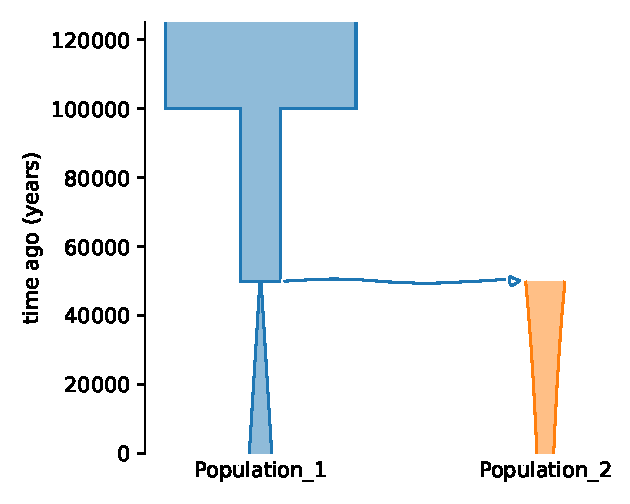
\includegraphics[width=\textwidth]{images_2/picture_2pops_str_3.pdf}
    \caption{}
    \label{fig:auto:struct_2_1_0_ex_2}
    \end{subfigure}%
    \begin{subfigure}[c]{.32\textwidth}
    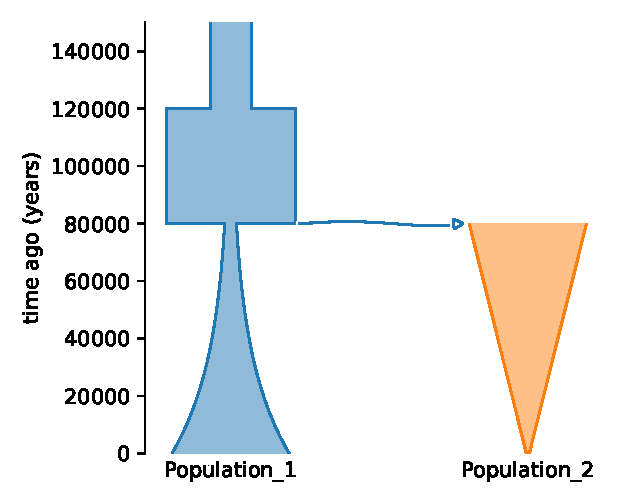
\includegraphics[width=\textwidth]{images_2/picture_2pops_str_4.pdf}
    \caption{}
    \label{fig:auto:struct_2_1_0_ex_3}
    \end{subfigure}
    \caption{Демографические истории для модели, представленной на рисунке~\ref{fig:auto:struct_2_1_0}, при разных значениях ее параметров}
    \label{fig:auto:struct_2_1_0_ex}
\end{figure}

\FloatBarrier
\textbf{Изменение модели демографической истории.}
Для изменения модели в разработанном методе автоматического перебора, был предложен метод увеличения числа временных интервалов в ограничении модели:
\begin{itemize}
    \item из трех частей временной оси (до первого разделения, между первым и вторым разделениями, после второго разделения) случайным образом выбрать часть, где еще не достигнуто финальное число временных интервалов;
    \item случайным образом выбрать временной интервал в части;
    \item разделить временной интервал на две части, создать новые параметры, вычислить их значения в соответствии со значениями старых параметров.
\end{itemize}

Опишем разработанный метод автоматического перебора моделей с использованием введенных понятий ограничений.
На первом шаге создается модель с числом временных интервалов, определенным минимальным ограничением $S_{\min}$, и осуществляется настройка ее параметров.
Затем на каждом последующем шаге увеличивается число временных интервалов в модели, и производится настройка параметров для модели с большим числом параметров.
Процесс завершается, когда найдены оптимальные параметры для модели с числом временных интервалов, которое соответствует максимальному ограничению $S_{\max}$.
На последнем шаге происходит сравнение моделей с разными структурами с использованием статистического критерия Акаике.\\

Вход:
\begin{itemize}
    \item генетические данные и информация о наличии зависимости в данных;
    \item набор булевых констант $B$, которые определяют какие параметры будут включены в модели;
    \item минимальное ограничение $S_{\min}$;
    \item максимальное ограничение $S_{\max}$.
\end{itemize}

Выход:
\begin{itemize}
    \item оптимальные значения параметров для моделей, соответствующих разным ограничениям;
    \item информация о лучшей модели при сравнении с использованием информационного критерия Акаике.
\end{itemize}

\begin{algorithm}
\caption{Процедура изменения модели для метода автоматического перебора}\label{alg:increase}
\begin{algorithmic}[1]
\Function{ChangeModel}{$\mathcal{M}, \theta^\star, S_{\text{cur}}, S_{\text{max}}, B$}
\State $D \leftarrow \{S^F[i] - S^*[i] \}_{i=1}^P$ \Comment{Ищем где можно увеличить число временных интервалов}
\State $Q \leftarrow $ \Call{DiscreteRandom}{$\{i\}_{i=1}^P, D$}
\State $d \leftarrow \sum_{i=1}^Q S^*[i] + $ \Call{UniformRandom}{$\{i\}_{i=1}^{S^*[Q]}$} \Comment{Выбираем индекс интервала}
\State $S_\text{cur}[Q] \leftarrow S_\text{cur}[Q] + 1$ \Comment{Новое число временных интервалов}
\State $\mathcal{M}_{\text{new}} \leftarrow \text{InsertTimeInterval}(\mathcal{M}, d)$ \Comment{Изменяем модель}
\State \Comment{Вычисляем значения параметров новой модели так, чтобы она соответствовала той же истории, что и предыдущая настроенная модель}
\State $\theta_{\text{new}} \leftarrow \text{GetParamsForSameHistory}(\mathcal{M}, \theta^\star, \mathcal{M}_\text{new})$
\State \Return $\mathcal{M}_\text{new}, \theta_\text{new}, S_\text{cur}$
\EndFunction
\end{algorithmic}
\end{algorithm}


\FloatBarrier
\subsection{Реализация разработанного метода автоматического перебора моделей расширенного класса}
\label{sec:part4:implementation}

Для реализации разработанного метода автоматического перебора моделей был разработан модуль \texttt{core}, который включает класс \texttt{CoreRun}, и был расширен модуль \texttt{models}.
Структура классов показана на рисунке~\ref{fig:part4:auto_method_impl}.

\begin{figure}[ht]
    \centering
    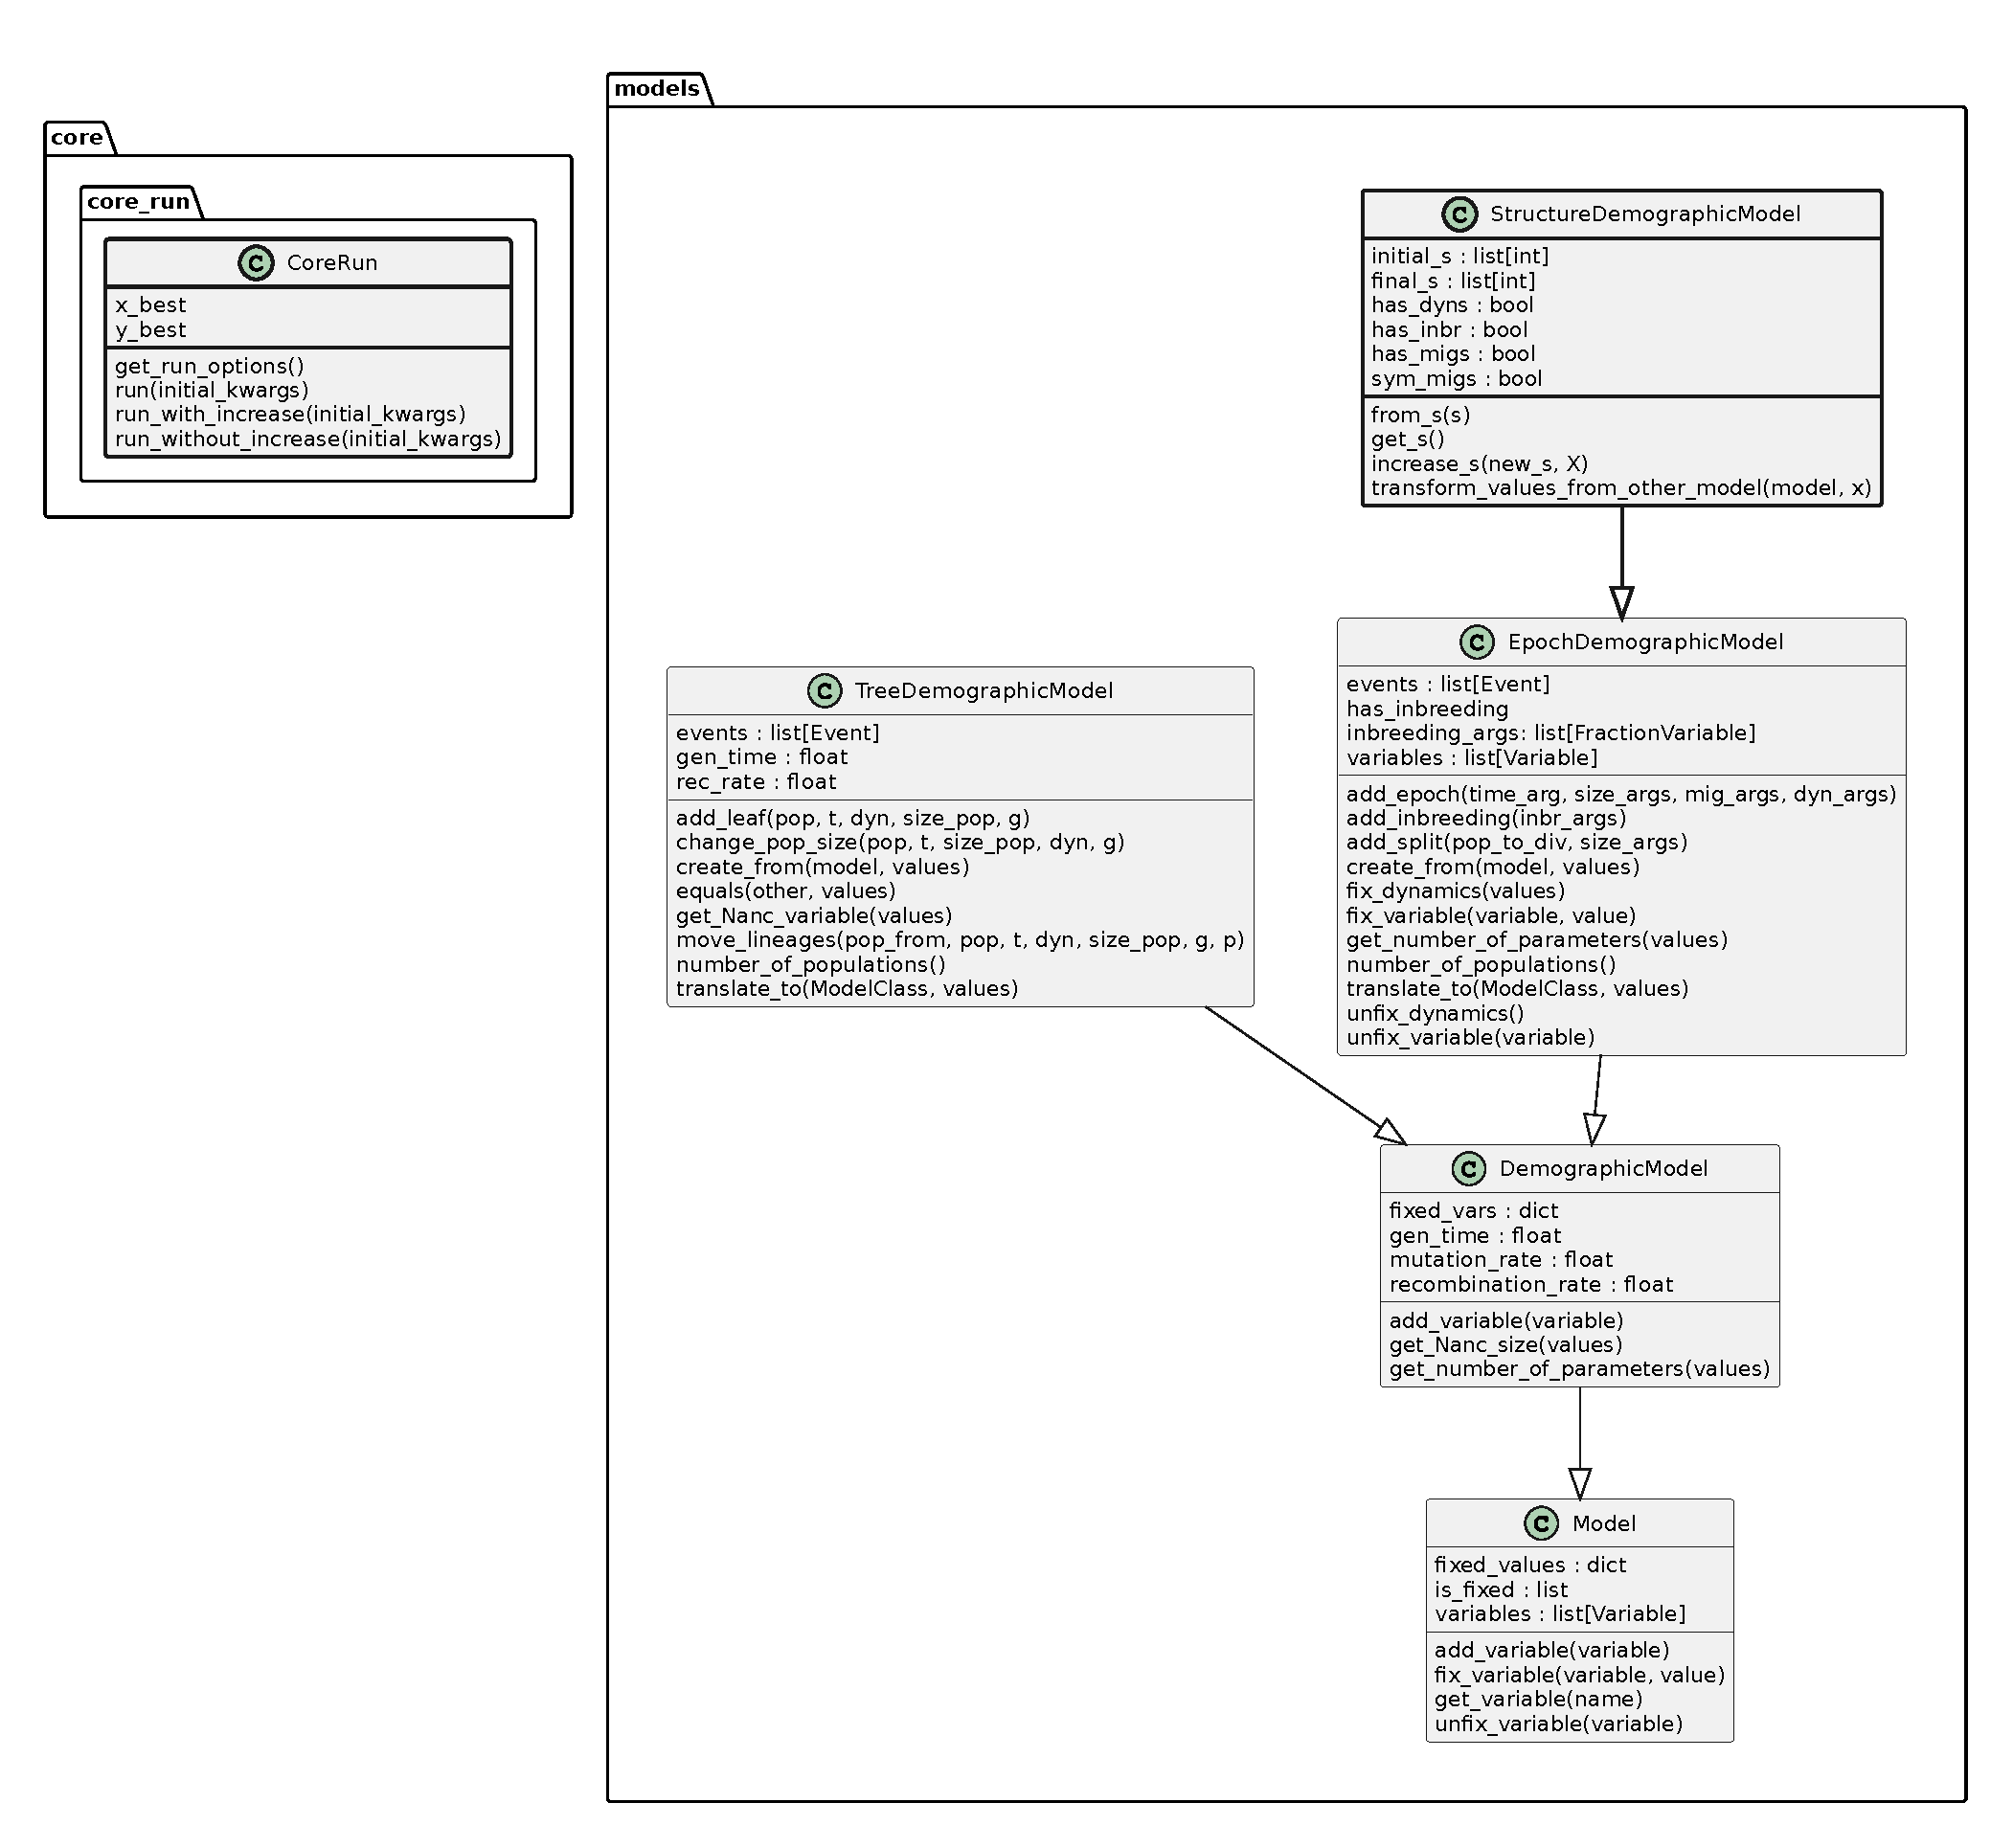
\includegraphics[width=0.97\linewidth]{images/part4/auto_model_implementation.pdf}
    \caption{Два класса, реализованных для разработанного метода автоматического перебора моделей}
    \label{fig:part4:auto_method_impl}
\end{figure}

В модуль \texttt{models} был добавлен новый класс  \linebreak \texttt{StructureDemographicModel}, который наследует класс \linebreak \texttt{EpochDemographicModel} расширенных моделей и описывает модели расширенного класса, определенные ограничением $S$ и набором булевых констант $B$.
Объект этого класса имеет следующие атрибуты:
\begin{itemize}
    \item \texttt{initial\_s} --- минимальное ограничение на число временных интервалов модели;
    \item \texttt{initial\_s} --- максимальное ограничение на число временных интервалов модели;
    \item \texttt{has\_dyns} --- набор булевых констант $\{b_\text{const}, b_\text{lin}, b_\text{exp}\}$, определяющих область определения параметров динамики;
    \item \texttt{has\_inbr} --- булева константа $b_\text{inr}$, определяющая наличие параметров инбридинга;
    \item \texttt{has\_migs} --- булева константа $b_\text{mig}$, определяющая наличие параметров миграции;
    \item \texttt{sim\_migs} --- булева константа $b_\text{sym\_mig}$, определяющая являются ли миграции симметричными.
\end{itemize}
У класса \texttt{StrcutureDemographicModel} реализованы четыре процедуры. Процедура \texttt{from\_s(s)} строит модель с числом интервалов, равным ограничению \texttt{s}.
Процедура \texttt{get\_s(s)} возвращает число временных интервалов между разделениями популяций в модели.
Остальные две процедуры реализуют важные части разработанного метода автоматического перебора.
Процедура \texttt{increase\_s(s)} производит изменение модели и увеличение числа временных интервалов --- процедура ChangeModel в псевдокоде.
Последняя процедура \texttt{transform\_values\_from\_other\_model} позволяет вычислить параметры модели по значениям вложенной модели таким образом, чтобы обе соответствовали одной демографической истории --- процедура GetParamsForSameHistory в псевдокоде.

Новый модуль \texttt{core} содержит единственный класс \texttt{CoreRun}, который реализует разработанный метод автоматического перебора моделей.
Метод реализован в процедуре \texttt{run\_with\_increase}, которая принимает на вход аргументы запуска, включающие генетические данные, метод вычисления правдоподобия и ограничения моделей, и возвращает настроенную модель, которая имеет максимальное значение критерия Акаике.

\FloatBarrier
\section{Экспериментальные исследования разработанного метода автоматического перебора моделей расширенного класса}
\label{sec:part4:experiments}

В данном разделе представлены проведенные экспериментальные исследования по выводу демографической истории популяций с помощью разработанного метода автоматического перебора расширенных моделей.

Используемые методы вычисления правдоподобия используют статистики генетических данных, которые могут являться довольно ограниченным источником информации~\cite{beichman2018using}.
Например, предыдущие исследования показали, что аллель-частотный одной популяции может соответствовать различным демографическим сценариям~\cite{myers2008can,rosen2018geometry}.
Проведенные экспериментальные исследования в разделе~\ref{sec:part2:experiments:genetic_algorithm:simulated_data} также подтверждают эти результаты.
Чем больше параметров содержат модели, тем больше шансы найти ложную демографическую историю при использовании аллель-частотного спектра.
Поэтому в проведенных экспериментальных исследованиях рассмотрены довольно ограниченные модели.
Однако разработанный метод может быть использован в будущем с более широкими ограничениями на модели при анализе более надежных данных.

\subsection{Вывод демографической истории трех популяций современного человека}

Одной из наиболее популярных демографических историй человеческих популяций является так называемая история «выхода из Африки» для трех популяций~\cite{gutenkunst2009inferring, jouganous2017inferring, harris2013inferring}:
\begin{itemize}
    \item YRI --- представители народа Йоруба из Ибадана, Нигерия;
    \item CEU --- европейская популяция, представленная жителями штата Юта с предками из Северной и Западной Европы;
    \item CHB --- представители народа Хань из Пекина, Китай.
\end{itemize}

Разработанный метод автоматического перебора моделей демографической истории был применен на данных этих трех популяций, ранее проанализированных в~\cite{gutenkunst2009inferring}.
В качестве метода вычисления правдоподобия был использован метод, реализованный в \dadi с размером сетки $pts=\{40, 50, 60\}$.
На рисунке~\ref{fig:part4:experiments:3pop_human:data_and_model} представлены данные и демографическая история, полученная по этим данным в работе~\cite{gutenkunst2009inferring}.
В работе~\cite{gutenkunst2009inferring} была настроена модель демографической истории с 13 параметрами с помощью множественных запусков локальной оптимизации.
Размер популяции YRI в использованной модели был представлен как два интервала константной численности, миграции были симметричными, а динамики изменения численности были равны константным, за исключением последнего временного интервала для популяций CEU и CHB, где был выбран экспоненциальный рост.

Аллель-частотный спектр размера $21 \times 21 \times 21$ был построен в работе~\cite{gutenkunst2009inferring} на основе данных из~\cite{sharp2000environmental} (рисунок~\ref{fig:part4:experiments:3pop_human:data}).
Данные включали мутации всех биаллельных позиций из некодирующих областей 219 генов.
Общая длина последовательности составила $4{,}04\cdot 10^6$ пар оснований.
Скорость мутации была выбрана, равной $2{,}35 \cdot 10^{-8}$ на позицию на поколение, как было использовано в~\cite{gutenkunst2009inferring}.
Для перевода времени в года было использовано среднее время одного поколения, равное 25 годам.

\begin{figure}[ht]
    \centering
    \begin{subfigure}[b]{0.4\linewidth}
        \centering
        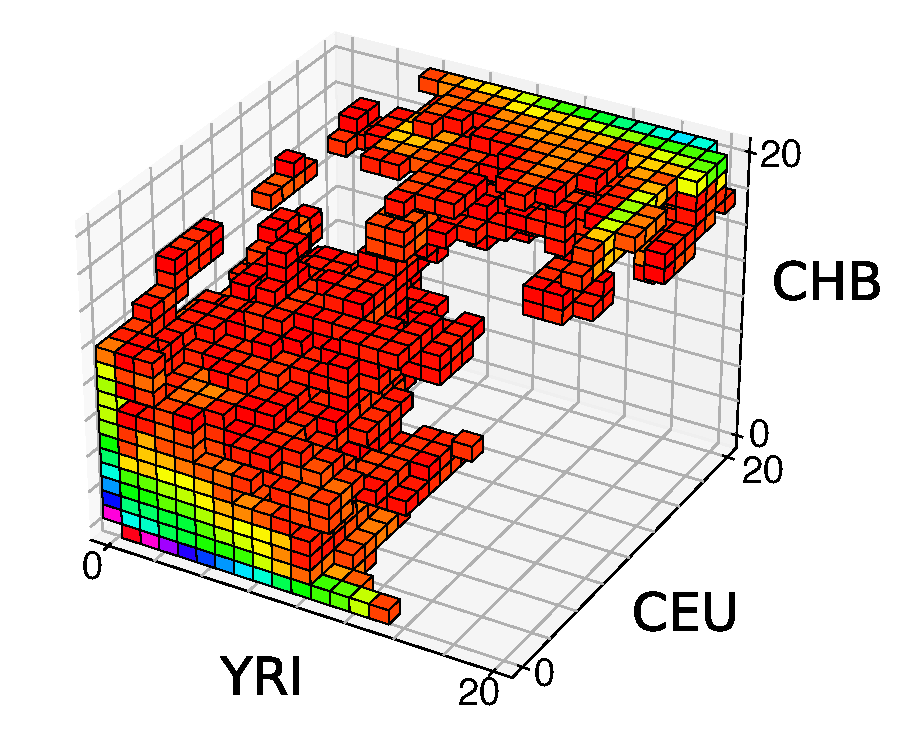
\includegraphics[width=\textwidth]{images_experiments/3pop_human_gutenkunst/3d_plot_fixed.pdf}
        \caption{}
        \label{fig:part4:experiments:3pop_human:data}
    \end{subfigure}
    \begin{subfigure}[b]{0.59\linewidth}
        \centering
        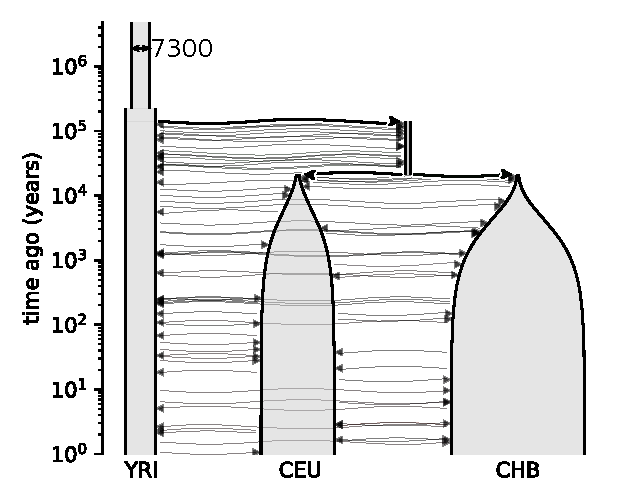
\includegraphics[width=\textwidth]{images_experiments/3pop_human_gutenkunst/picture_3pop_guten.pdf}
        \caption{}
        \label{fig:part4:experiments:3pop_human:model}
    \end{subfigure}
    \caption{Генетические данные в виде аллель-частотного спектра и демографическая история, полученная ранее в работе~\cite{gutenkunst2009inferring}}
    \label{fig:part4:experiments:3pop_human:data_and_model}
\end{figure}

Для применения разработанного метода автоматического перебора моделей требуется определить минимальные и максимальные ограничения.
Так как был использован метод на основе аллель-частотного спектра, ограничения на число временных интервалов в моделях были выбраны небольшими.
Минимальное ограничение было равно (1,1,1), что означает один временной интервал до первого разделения популяции, один интервал между первым и вторым разделениями популяций и один --- после второго.
Максимальное ограничение было выбрано равным (2,1,1), что описывает модель с двумя интервалами до первого разделения, с одним интервалом между первым и вторым разделениями и одним интервалом после второго разделения.
Таким образом, метод перебирал только две возможные модели --- модель 1 и модель 2, соответствующие минимальному и максимальному ограничению.

Настроенные параметры моделей, наилучшие значения правдоподобия, а также информационного критерия Акаике (CLAIC) могут быть найдены в работе~\cite{noskova2020gadma} в таблице~3.
Согласно этим результатам~\cite{noskova2020gadma}, наилучшая демографическая история была получена для модели, соответствующей ограничению (2,1,1) на число интервалов.
На рисунке~\ref{fig:part4:experiments:3pop_human:result} представлено сравнение настроенной модели с результатом, полученным ранее в~\cite{gutenkunst2009inferring}.
Полученная демографическая история имеет больше параметров, чем модель, использованная в~\cite{gutenkunst2009inferring}: 20 непрерывных параметров против 13.
Несмотря на это информационный критерий Акаике (CLAIC) выделяет модель, полученную разработанным методом, как наилучшую.
Демографические истории, полученные разработанным методом и в работе~\cite{gutenkunst2009inferring}, весьма схожи.
Значения современных размеров европейской (CEU) и азиатской (CHB) популяций были получены немного меньше, чем ранее.
Основными отличиями, однако, являются значения интенсивностей миграций и численность общей евразийской популяции, которая экспоненциально растет с $200$ до $1{\,}500$ особей.
Для сравнения в истории из~\cite{gutenkunst2009inferring} эта численность является константной, равной $2{\,}000$ особей, что является чуть менее реалистичным, чем экспоненциальный рост.
Интенсивности миграций в полученном результате являются асимметричными и имеют значения выше, чем в истории, найденной в~\cite{gutenkunst2009inferring}.
Наиболее интенсивная миграция произошла между популяциями YRI и CEU, а после второго разделения --- между популяциями CEU и CHB.
Отметим, что интенсивности миграций соотносятся с известным географическим положением: чем более географически удалены друг от друга популяции, тем меньше полученная интенсивность миграции. 
\begin{figure}[ht]
    \centering
        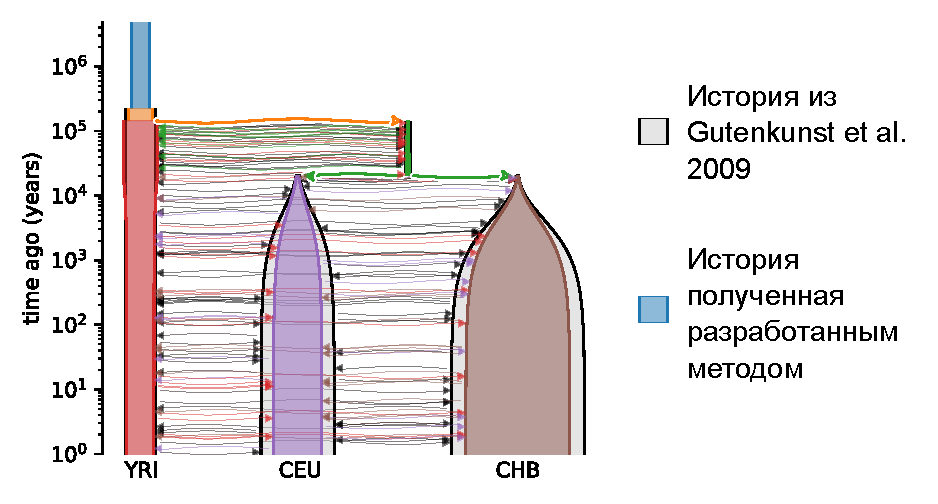
\includegraphics[width=0.8\textwidth]{images_experiments/3pop_human_gutenkunst/picture_3pop_result.pdf}
    \caption{Демографическая история, полученная разработанным методом}
    \label{fig:part4:experiments:3pop_human:result}
\end{figure}

\subsection{Вывод демографической истории популяций кошачьей лягушки}

Разработанный метод автоматического перебора моделей демографической истории был использован для вывода демографических историй популяций кошачьей лягушки.
В работе~\cite{portik2017evaluating} были представлены генетические данные в виде аллель-частотного спектра для трех пар популяций, а также был выполнен ручной перебор моделей.
При построении данных генетические данные были отобраны и только независимые позиции были использованы.
Как следствие модели с разным числом параметров можно корректно сравнивать с помощью информационного критерия Акаике~\cite{akaike1974new}.

Рассматриваемые данные кошачьей лягушки были ранее проанализированы во второй главе в разделе~\ref{part2:frogs} в экспериментальных исследованиях разработанного метода настройки параметров моделей на основе генетического алгоритма.
Для всех моделей, ранее настроенных в статье~\cite{portik2017evaluating}, экспериментальные исследования позволили получить параметры, обеспечивающие лучшее значение правдоподобия.

В этом разделе представлены результаты экспериментальных исследований применения метода автоматического перебора моделей.
Метод был применен для вывода демографической истории трех пар популяций: 1) северная (Northern) и южная (Southern) популяции; 2) популяции CVLN и CVLS; и 3) популяции CrossRiver и CVLN.
Минимальное ограничение на модели было выбрано равным одному временному интервалу до разделения и одному временному интервалу после разделения популяций.
Максимальное ограничение составило два временных интервала до разделения и три временных интервала после разделения популяций.
Модели были сравнены с использованием информационного критерия Акаике (AIC).

Результаты представлены в работе~\cite{noskova2020gadma} в таблице~S2 для популяций Northern, Southern, в таблице~S3 для популяций CVLN, CVLS, в таблице~S4 для популяций CrossRiver, CVLN.
полученные демографические истории изображены на рисунке~\ref{fig:part3:experiments:frog:results}.

\begin{figure}[ht]
    \centering
    \begin{subfigure}[b]{.33\textwidth}
    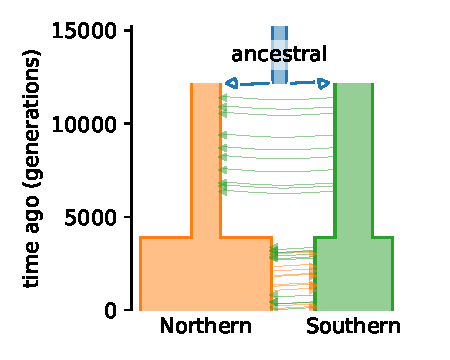
\includegraphics[width=\textwidth]{images_experiments/gaboon_forest_frog/auto/picture_1pop_model_nor_sou.pdf}
    %\caption{}
    \label{fig:part3:experiments:frog:results_1}
    \end{subfigure}%
    \begin{subfigure}[b]{.33\textwidth}
    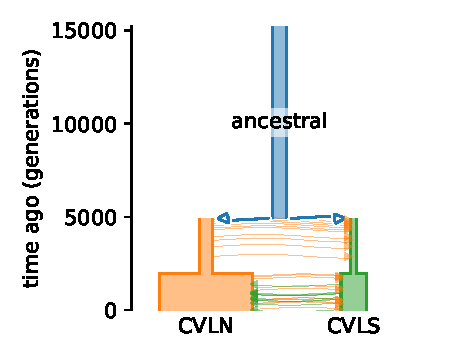
\includegraphics[width=\textwidth]{images_experiments/gaboon_forest_frog/auto/picture_1pop_model_cvln_cvls.pdf}
    %\caption{}
    \label{fig:part3:experiments:frog:results_2}
    \end{subfigure}%
    \begin{subfigure}[b]{.33\textwidth}
    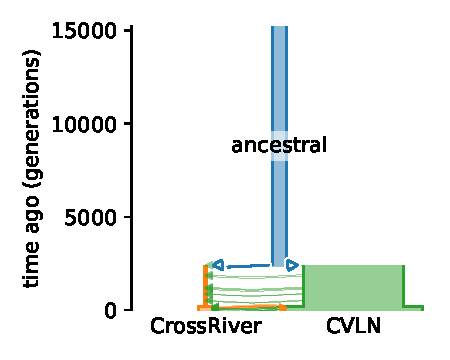
\includegraphics[width=\textwidth]{images_experiments/gaboon_forest_frog/auto/picture_1pop_model_cross_cvln.pdf}
    %\caption{}
    \label{fig:part3:experiments:frog:results_3}
    \end{subfigure}
    \caption{Полученные демографические истории для  различных пар популяций кошачьей лягушки}
    \label{fig:part3:experiments:frog:results}
\end{figure}

Все демографические истории популяций кошачьей лягушки, полученные разработанным методом автоматического перебора, имеют один временной интервал до разделения и два интервала после разделения предковой популяции.
Две из трех полученных демографических историй имеют наилучшие значения информационного критерия Акаике при сравнении с моделями, перебранными вручную в работе~\cite{portik2017evaluating} (таблицы~S2~и~S4 в работе~\cite{noskova2020gadma}).
Для данных популяций CVLN и CVLS демографическая история, полученная методом автоматического перебора, имеет значение AIC хуже, чем наилучшая модель, полученная ручным перебором в~\cite{portik2017evaluating}.
Однако заметим, что на основании этой модели, построенной автоматически, можно рассмотреть аналогичную модель с исключенным параметром миграции из популяции CVLS в популяцию CVLN.
Для такой вложенной модели значение информационного критерия Акаике будет равно $926.2$, что является наилучшим значением среди всех ранее полученных моделей.

Настроенные модели демонстрируют односторонние миграции во время первого временного интервала после разделения.
Наличие одного интервала до разделения предковой популяции и двух интервалов после разделения согласуется с результатами, полученными в~\cite{portik2017evaluating}.
Таким образом, разработанный метод автоматического перебора моделей позволил построить и настроить модели демографических историй, обеспечивающих наилучшее значение правдоподобия, чем было получено ранее с использованием ручного перебора.

\subsection{Вывод демографической истории двух и трех популяций голубой акулы}

Разработанный метод автоматического перебора моделей был использован для вывода демографической истории популяций голубых акул.
Генетические данные включали полногеномные последовательности 376 особей (рисунок~\ref{fig:part2:experiments:blue_shark:geogr}).
Было выделено три популяции, представленные в этих данных:
\begin{itemize}
    \item северная популяция (Northern) --- север Атлантического океана и Средиземное море:
    \item южная популяция (Southern) --- Индийский океан и юго-западная часть Тихого океана;
    \item южноафриканская популяция (SAF).
\end{itemize}

\begin{figure}[ht]
    \centering
        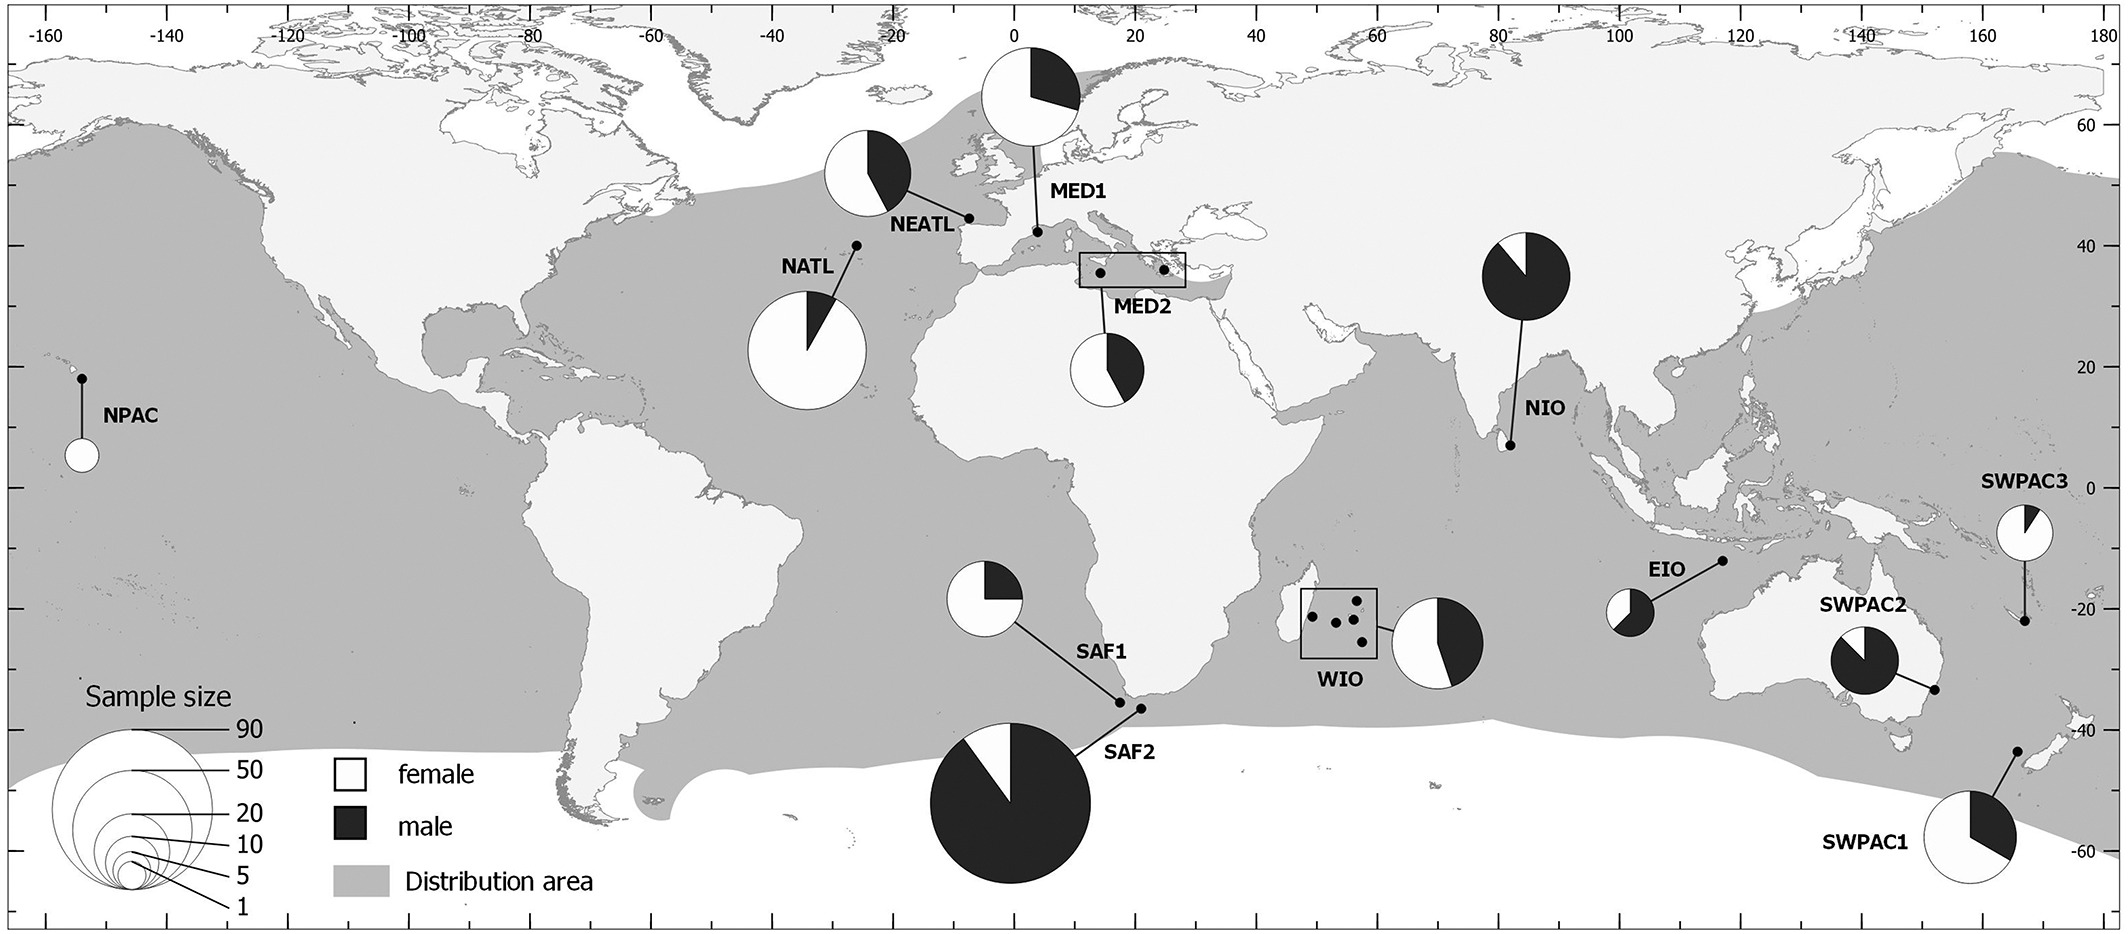
\includegraphics[width=\linewidth]{images_experiments/blue_shark/from_paper.jpg}
    \caption{Географическое расположение образцов генетических данных. Источник: \cite{nikolic2022stepping}}
    \label{fig:part2:experiments:blue_shark:geogr}
\end{figure}

На основе генетических данных были построены несколько аллель-частотных спектров, представленных на рисунке~\ref{fig:part4:experiments:blue_shark:data}.
Для вывода демографической истории были построены три спектра.
Первый спектр для двух популяций (рисунок~\ref{fig:part4:experiments:blue_shark:data_1}) размера $51\times51$ был использован для вывода демографической истории северной и южной популяций.
Для вывода демографической истории трех популяций было использовано два спектра разного размера: $21\times21\times21$ (рисунок~\ref{fig:part4:experiments:blue_shark:data_2}) и $51\times51\times51$ (рисунок~\ref{fig:part4:experiments:blue_shark:data_3}).

\begin{figure}[ht]
    \centering
    \begin{subfigure}[b]{0.4\linewidth}
        \centering
        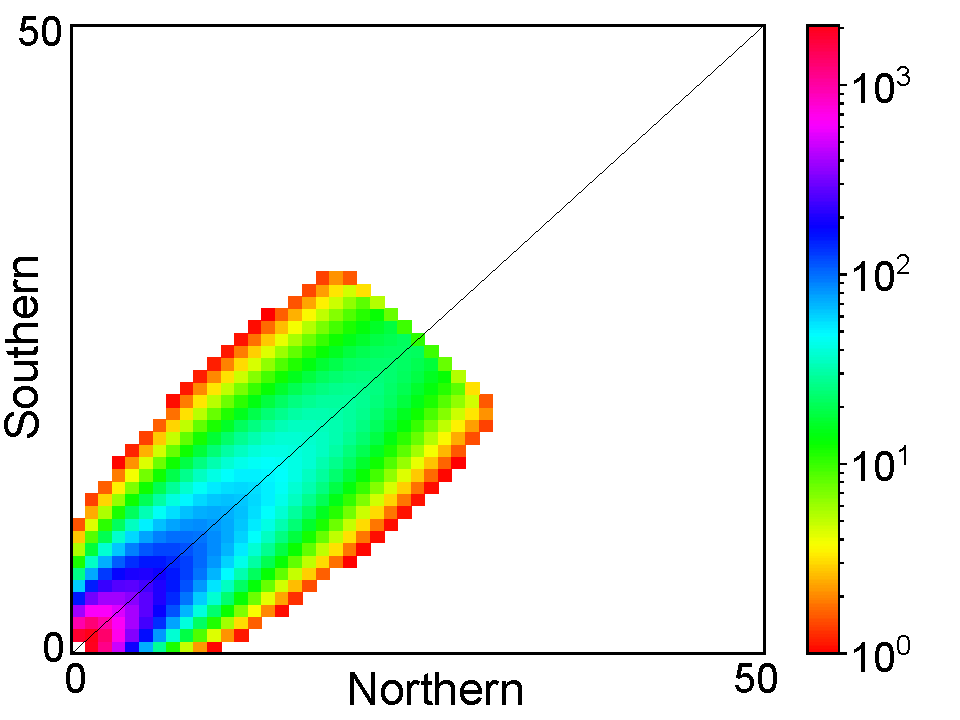
\includegraphics[width=\textwidth]{images_experiments/blue_shark/2pop_afs.pdf}
        \caption{}
        \label{fig:part4:experiments:blue_shark:data_1}
    \end{subfigure}
    \begin{subfigure}[b]{0.4\linewidth}
        \centering
        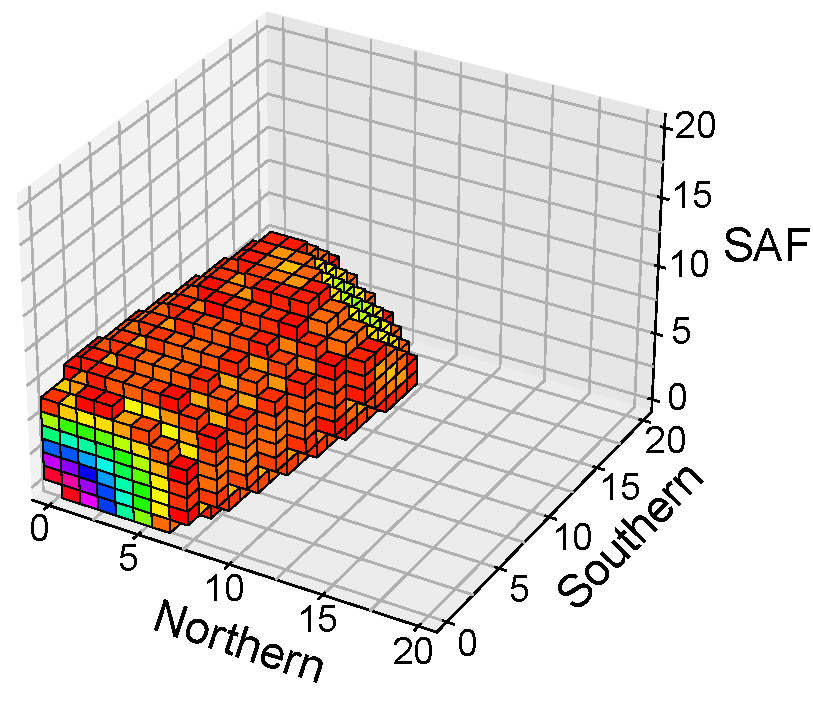
\includegraphics[width=\textwidth]{images_experiments/blue_shark/3pop_afs_20.pdf}
        \caption{}
        \label{fig:part4:experiments:blue_shark:data_2}
    \end{subfigure}%
    \begin{subfigure}[b]{0.4\linewidth}
        \centering
        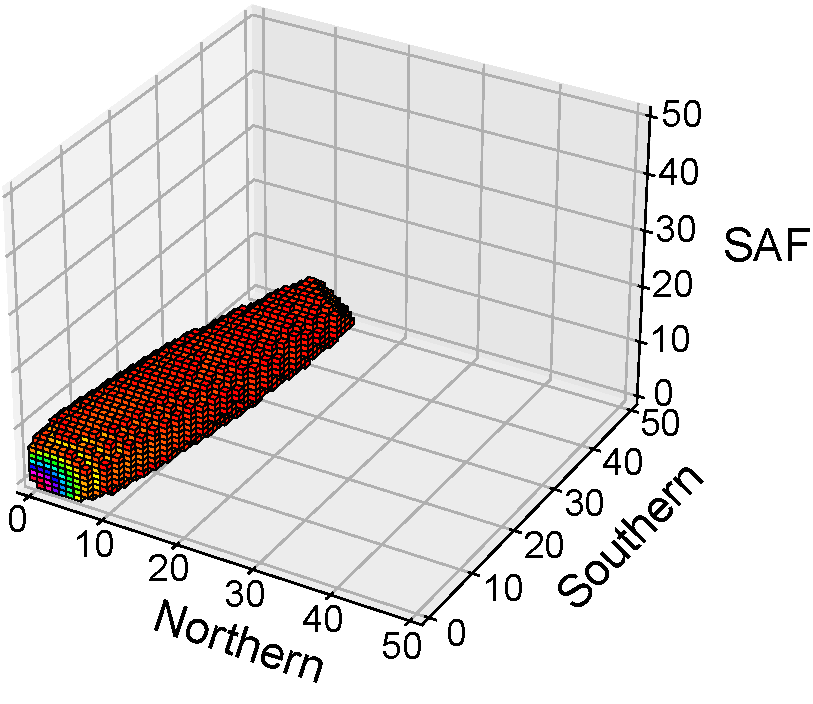
\includegraphics[width=\textwidth]{images_experiments/blue_shark/3pop_afs_50.pdf}
        \caption{}
        \label{fig:part4:experiments:blue_shark:data_3}
    \end{subfigure}
    \caption{Генетические данные в виде аллель-частотных спектров для (а) двух популяций, (б) и (в) трех популяций}
    \label{fig:part4:experiments:blue_shark:data}
\end{figure}

Для вывода демографической истории популяций был использован метод вычисления правдоподобия, реализованный в \moments.
Каждая настройка параметров была повторена 50 раз и выбраны лучшие результаты.
Скорость мутаций была выбрана, равной $10^{-8}$ на позицию на поколение~\cite{pirog2018structure, duncan2006global}, длина генома составила $2{\,}598{\,}195$ пар оснований~\cite{rougeux2017modeling}.
Для перевода значений параметров времени из поколений в года было использовано среднее время одного поколения, равное девяти годам, поскольку ранее опубликованные оценки составляли $8{,}1$ лет~\cite{poisson2007compilation} и $8{,}2$, $9{,}8$ лет~\cite{cortes2010ecological} для южноафриканской и северной популяций.

Для вывода демографической истории популяций голубой акулы был разработан многоступенчатый подход, схема которого изображена на рисунке~\ref{fig:part2:experiments:blue_shark:scheme}.
Сначала, был применен разработанный метод автоматического перебора расширенных моделей для вывода демографической истории северной (Northern) и южной (Southern) популяций по аллель-частотному спектру, представленному на рисунке~\ref{fig:part4:experiments:blue_shark:data_1}.
Этот шаг позволяет автоматически перебрать модели, а также настроить динамики изменения численности популяций.

\begin{figure}[ht]
    \centering
        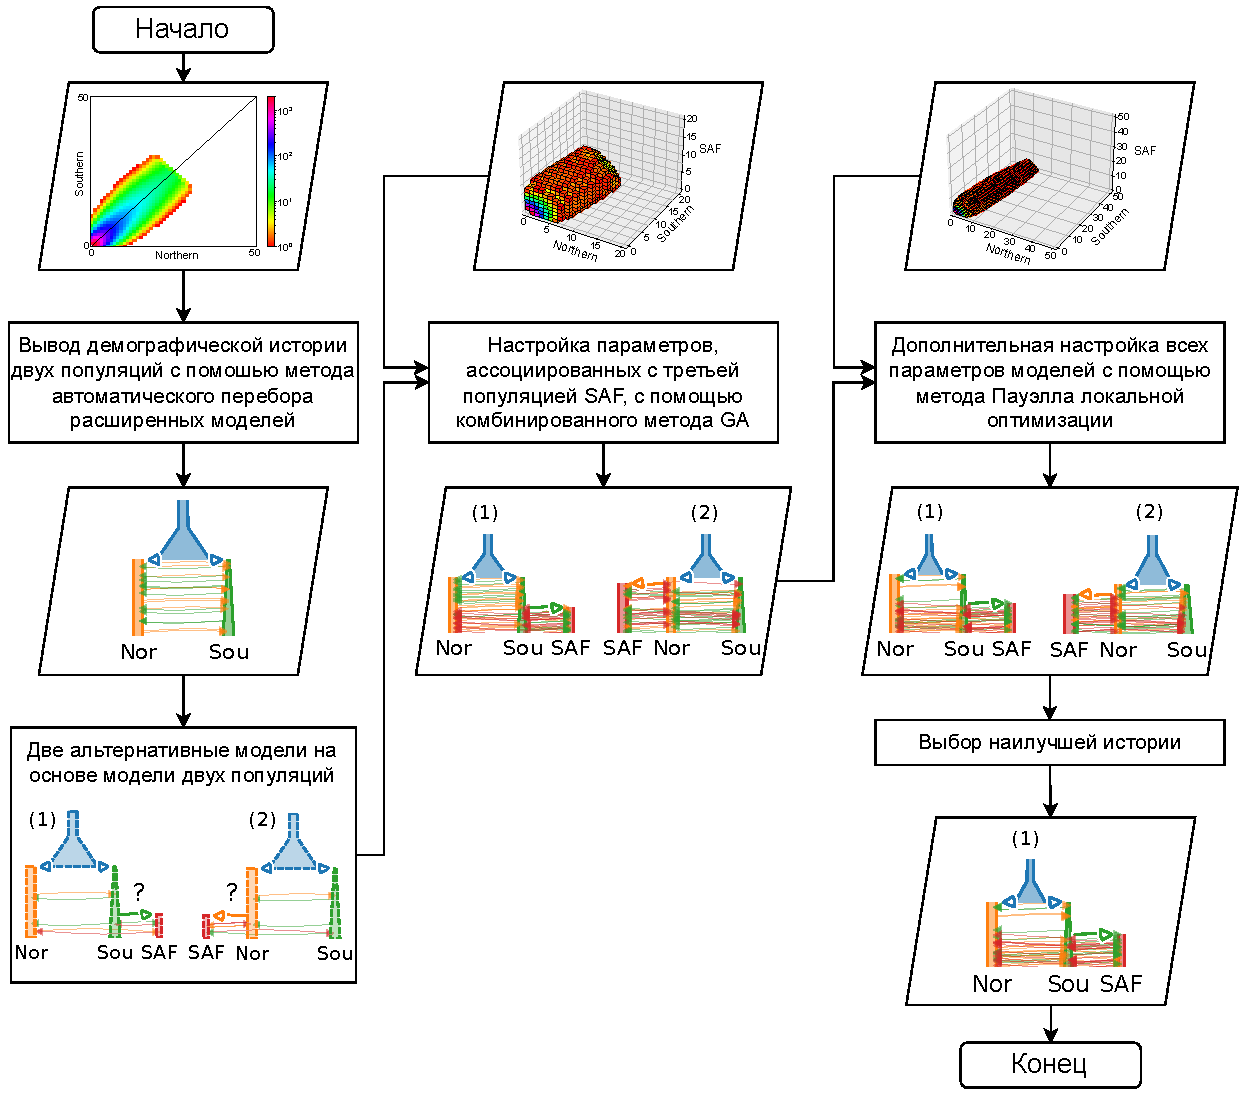
\includegraphics[width=\linewidth]{images_experiments/blue_shark/blue_shark_scheme.drawio.pdf}
    \caption{Схема вывода демографической истории популяций голубой акулы}
    \label{fig:part2:experiments:blue_shark:scheme}
\end{figure}

Затем, наилучшая модель двух популяций была модифицирована и третья популяция была добавлена.
Было рассмотрено две модифицированные модели: 1) модель 1, в которой южноафриканская популяция SAF отделилась от южной популяции Southern, 2) модель 2, в которой южноафриканская популяция SAF отделилась от северной популяции Northern.
Численность южноафриканской популяции была выбрана постоянной, было добавлено семь новых параметров.
Для увеличения точности финальных результатов настройка параметров двух модифицированных моделей трех популяций была произведена в два этапа.
На первом этапе все параметры, ассоциированные с моделью двух популяций, были фиксированы.
С помощью разработанного метода на основе комбинации генетического алгоритма и метода Пауэлла локальной оптимизации была выполнена настройка семи новых параметров, ассоциированных с историей южноафриканской популяции SAF.
Настройка была проведена по аллель-частотному спектру размера $21\times21\times21$, представленному на рисунке~\ref{fig:part4:experiments:blue_shark:data_2}.
На втором этапе настройка была проведена для всех параметров моделей с использованием метода Пауэлла локальной оптимизации по аллель-частотному спектру размера $51\times51\times51$, представленному на рисунке~\ref{fig:part4:experiments:blue_shark:data_3}.
В конце две модели были сравнены по значению правдоподобия --- они имеют равное число параметров.

Для вывода демографической истории двух популяций был использован разработанный метод автоматического перебора моделей.
Были использованы следующие ограничения на модели: минимальное число временных интервалов --- (1,1,0), максимальное число временных интервалов --- (2,1,0).
Таким образом, метод перебирал только две модели.
Первая модель имела один временной интервал до разделения и один после.
Вторая модель включала два временных интервала до разделения и один после.
Такое малое число временных интервалов обусловлено ограниченными возможностями аллель-частотного спектра, указанными ранее.
Модели были сравнены с использованием модифицированного критерия Акаике (CLAIC), так как данные имели зависимости.

Результаты показали, что модель с двумя временными интервалами до разделения имеет лучшее значение CLAIC и, следовательно, лучше описывает генетические данные.
Финальная настроенная модель двух популяций представлена на рисунке~\ref{fig:part2:experiments:blue_shark:2pop_hist}.
Значения настроенных параметров могут быть найдены в работе~\cite{nikolic2022stepping} в таблице~4.
Численность предковой популяции составила около $30{\,}000$  особей, и она линейно росла до $170{\,}000$ особей, после чего разделилась на северную и южную популяции.
Этот линейный рост начался около $1{\,}170{\,}000$ лет назад, а разделение около $5{\,}000$ лет назад.
Северная популяция имела постоянную численность в $5{\,}000$ особей, а южная популяция имела слабый линейный рост численности от $4{\,}000$ особей в момент образования до $6{\,}000$ особей в настоящий момент.
Миграции между популяциями были асимметричные и миграция из южной популяции в северную гораздо интенсивнее миграции в обратном направлении.

\begin{figure}[ht]
    \centering
        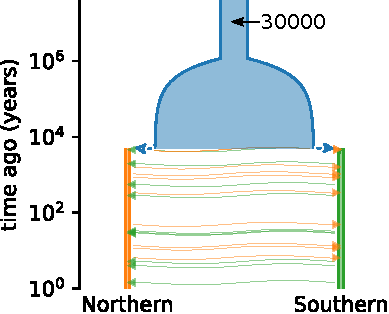
\includegraphics[width=0.4\linewidth]{images_experiments/blue_shark/2pop_history.pdf}
    \caption{Демографическая история двух популяций голубой акулы}
    \label{fig:part2:experiments:blue_shark:2pop_hist}
\end{figure}

Вывод демографической истории трех популяций с использованием двух модифицированных моделей и многоступенчатой настройки параметров показал, что модель 1 лучше описывает генетические данные, чем модель 2.
В частности, это означает, что южноафриканская популяция отделилась от южной популяции, а не от северной.
Рисунок лучшей демографической истории представлен на рисунке~\ref{fig:part2:experiments:blue_shark:2pop_hist}.
Настроенные параметры представлены в~\cite{nikolic2022stepping} в таблице~S7.

\begin{figure}[ht]
    \centering
        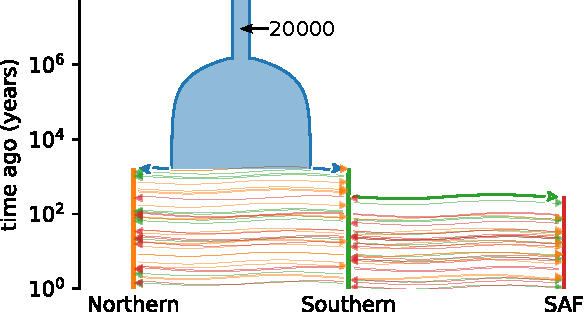
\includegraphics[width=0.6\linewidth]{images_experiments/blue_shark/3pop_history.pdf}
    \caption{Демографическая история трех популяций голубой акулы}
    \label{fig:part2:experiments:blue_shark:3pop_hist}
\end{figure}

История трех популяций немного отличается от истории двух популяций.
Отметим, что она является более надежной, так как включает больше популяций и учитывает больше генетических данных.
Размер предковой популяции составил $20{\,}000$ особей.
Эта численность начала линейно увеличиваться около $1{,}4$ миллиона лет назад и выросла до $165{\,}000$ особей.
Предковая популяция разделилась $1{\,}600$ лет назад на северную и южную популяции.
От южной популяции 300 лет назад отделилась южноафриканская популяция.
Численность северной популяции составила $2{\,}000$ особей, численность южной популяции выросла с $1{\,}500$ до $3{\,}000$ особей, а размер южноафриканской популяции оставался примерно постоянным около $1{\,}500$ особей.
Миграции между северной и южноафриканской популяциями отсутствовали.
Миграция из южноафриканской популяции в южную была самая интенсивная.

Согласно полученным результатам, линейный рост предковой популяции начался в раннем плейстоцене, а раскол на северную и южную популяции произошел во время эпохи голоцена.
Апробация результатов коллегами из области зоологии~\cite{nikolic2022stepping} позволила предположить, что палеоклиматические события спровоцировали расхождение северной и южной популяций.
В эпоху голоцена температура морской поверхности в тропиках имела тенденции к потеплению и так продолжалось до момента времени $5{\,}000$ лет назад.
После этого момента и до настоящего времени температура морской поверхности хоть и колебалась, но имела тенденцию к глобальной стабилизации.
Например, в работе~\cite{leduc2010holocene} было выявлено потепление примерно на $2^\circ C$ в западной тропической части Атлантического океана и восточной тропической части Тихого океана с раннего голоцена до настоящего времени.
Было выявлено глобальное похолодание в Северном полушарии около $5{\,}000$ лет назад~\cite{masson2013information}.

Записи озерных отложений из Гренландии также позволяют предположить, что около $4{\,}500$ и $650$ лет назад температура поверхности перестала нагреваться и начала колебаться, в том числе и в отрицательную сторону~\cite{masson2013information, olsen2012variability}.
Более того, это колебание температуры морской поверхности происходило и в Южном полушарии: было показано, что температура в австралийско-новозеландском регионе во время голоцена имела тенденцию к снижению~\cite{bostock2013review}, как и в Южном океане~\cite{kaiser2008glacial,shevenell2011holocene}.
Согласно полученным результатам разделение предковой популяции как раз произошло около $5{\,}000$ лет назад, когда произошло изменение тенденции изменения температуры.
Эти колебания температуры морской поверхности в прошлом могли способствовать разделению северной и южной популяций.
Сдвиги в сезонах размножения голубых акул между двумя полушариями могли способствовать сохранению этого разделения: в Северном полушарии размножение происходит летом (июль, август)~\cite{fujinami2017reproductive}, как и в юго-западной экваториальной части Атлантического океана~\cite{coelho2018distribution}, а в Индийском океане --- с октября по декабрь~\cite{druon2022global}.


Полученные демографические истории трех популяций показала, что численность голубых акул сильно сократилась при разделении предковой популяции: численность северной и южной популяций при разделении предковой популяции составили только 2--3\% от размера предковой популяции.
Кроме того, результаты показали довольно низкие современные размеры популяции.
Полученные размеры $4{\,}000$ -- $6{\,}000$ особей согласуются с оценками, полученными ранее в~\cite{verissimo2017world,king2015genetic}.


\section*{Выводы по граве~\ref{ch:auto_model}}
\addcontentsline{toc}{section}{Выводы по главе~\ref{ch:auto_model}}

\begin{enumerate}[label={\arabic*.}]
    \item Разработан метод автоматического перебора расширенных моделей демографической истории одной, двух и трех популяций по генетическим данным.
    \item Метод был применен для вывода демографической истории «выхода из Африки» для трех популяций современных людей. Полученная история имеет не только лучшее значение правдоподобия, чем ранее полученная история по тем же данным, но и лучшее значение информационного критерия Акаике. Результаты согласуется с другими исследованиями.
    \item Метод был применен для вывода демографической истории трех пар популяций кошачьей лягушки.
    Полученные демографические истории имеет не только лучшее значение правдоподобия, чем истории, ранее полученные по тем же данным ручным перебором моделей, но и лучшие значения информационного критерия Акаике.
    \item Выведена демографическая история трех популяций голубой акулы по данным, которые ранее не были проанализированы. Полученная демографическая история согласуется с другими исследованиями этого биологического вида.
\end{enumerate}